Research in high energy physics typically requires hadron colliders such as the Tevatron and the LHC as they can produce extremely high energies through proton-proton collisions. These collisions produce heavy particles with extremely short lifespans such as the top quark and W-bosons, making an ideal environment to study properties of heavy particles. This includes searches beyond the SM with SUSY and its sparticles. Located on the border of France and Switzerland, the LHC is the current world-leading facility for high energy physics collider experiments. The primary experimental collaboration for SUSY phenomena is the ATLAS (A Toroidal LHC ApparatuS) \cite{collaboration2008atlas} and CMS (Compact Muon Solenoid) \cite{chatrchyan2008cms} collaborations, where both collaborations at the LHC work independently of each other.

%-------------------------------------------------------------------------%
\section{The Large Hadron Collider and CMS}
The LHC currently operates at $ \sqrt{s}=13 \text{TeV} $, where the energy is $5-6$TeV higher than when the Higgs Boson was discovered. ATLAS and CMS are the general multi-purpose detectors at the LHC that conduct independent searches of high energy physics. Each detector is built slightly differently, allowing for variability in detection (although not too varying) to support any discoveries made at the LHC. \\

The CMS detector \cite{chatrchyan2008cms} weighs $12.5\times10^6$kg with a solenoid of 4T AND WRITE ABOUT PARAMETERS HERE. CMS has focused on a single large superconducting magnet. These detection parameters will be useful when considering kinematic variables associated importantly to stop production, just as it was for SM particle productions.

%-------------------------------------------------------------------------%
\section{Simulations of a collider}
Data collected in colliders do not initially contain a label regarding which physical process the entry corresponds to. A method to overcome this may be to individually observe each event and provide a corresponding label provided the correct understanding of the physics behind such processes. However, this is evidently inefficient and unrealistic. By performing simulations identical to the properties of the particle collider and closely following the production process with known theory and calculations, one may identify the process in the raw data using techniques such as ML. One program of such is MadGraph5 (MG5) \cite{alwall2014automated, alwall2011madgraph}, where the next-to-leading order differential cross-sections of an input event are generated at tree-level with Monte Carlo simulations. \\

The processes generated by MadGraph are known to be ``generator level", meaning the processes are only produced to what we specify it as, disregarding any physics that follow. Consequently, the events do not mimic an output of the detector exactly. In order to achieve a high resolution of detector simulations, these events must be processed further into what a real detector may observe. \\

%\section{Parton Showers with Pythia and detector simulation with Delphes}
A program called PYTHIA8.2 \cite{sjostrand2015introduction}has the functionality to extend the decays produced by MadGraph in a physical process known as parton showers. Intended to describe all components - such as elastic, diffractive, and non-diffractive topologies - of the total cross-section in collisions for soft processes, PYTHIA also includes capabilities such as \textit{parton distributions}, \textit{parton showers}, \textit{multi-parton interactions} and its own \textit{hard processes} such as QCD, electroweak and SUSY processes. Multi-parton interactions are not necessarily relevant to maintain in our processes, so by turning this feature off we save computation time. \\
%The user manual and website for the latest release (PYTHIA8.2) is recommended for readers who are interested in the specifics \cite{sjostrand2015introduction}, although more comprehensive physics are stated in the older version PYTHIA6.4. 

Delphes is the detector level simulation chosen for this project, due to its MadGraph build-in making the generation process smooth. The package allows us to choose either the ATLAS or CMS detector to simulate, in which CMS was chosen due to our parameters following those of CMS papers.


%-------------------------------------------------------------------------%
\section{Kinematic variables in collider experiments}
Data at the LHC is collected by taking measurements of the properties of particles resultant particles in the transverse plane to the beam direction. Considering the beam direction to be the z-direction the transverse plane would be the $(x,y)$-plane, with the geometry of this depicted in Figure \ref{fig:beam}. \\

\begin{figure}[htbp]
    \centering
    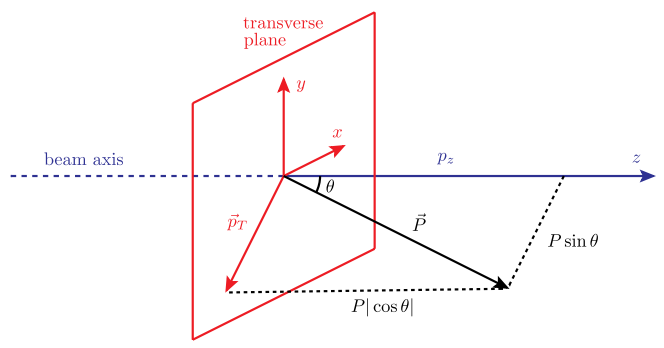
\includegraphics[width=12cm, height= 6cm]{beam.png}
    \caption{The geometry of a collider experiment, with the beam axis considered as the z-direction and the transverse plane as the $(x,y)$-plane \cite{barr2011guide}.}
    \label{fig:beam}
\end{figure}


A well summarized guide to the transverse plane and variables considered is given in reference \cite{barr2011guide}, where there are three types of projection methods - \textit{Mass-preserving}, \textit{Speed-preserving} and \textit{Massless}. The principal component being the transverse momentum given by Equation (\ref{eq:pt})
\begin{equation}
    p_T = \sqrt{p_x^2 + p_y^2}
    \label{eq:pt}
\end{equation}
maintains equivalence across the three types, the mass projections defer between the three. \\

An important variable to discriminate background and signals in collider experiments is the \textit{missing transverse energy} denoted as $\cancel{\it{E}}_{T}$, where it is, in general, the negative of the vector sum of the $p_T$ components reconstructed in the detector \cite{cms2011missing}. In the SM decays, leptonic decays produce their neutrino counterparts that freely passes through the detector, resulting in some $\cancel{\it{E}}_{T}$. Many SUSY events are predicted to have a large excess of $\cancel{\it{E}}_{T}$ moreso than the SM processes, due to a larger excess of undetectable particles. The reconstruction of the $\cancel{\it{E}}_{T}$ is sensitive to slight deviations such as mismeasurements and cosmic-ray particles.  %One may also consider the \textit{stransverse mass} denoted as $M_{T2}$ when searching for particles beyond SM. This observable places a maximal lower bound on the almost-invisible parent particles that decayed into detected particles \cite{lester2011stransverse}. These are only a few of many variables that could be used for analyses and will require further reading and careful exploration for potential candidates for the project.



%-------------------------------------------------------------------------%
\section{Possible search regions for the top squarks}


\begin{equation}
 pp \rightarrow t \Bar{t} \rightarrow b\Bar{b}jjl\cancel{\it{E}}_{T},
 \label{eq:background}
\end{equation}
\begin{equation}
  pp \rightarrow \Tilde{t}\Tilde{t^*} \rightarrow t \Bar{t} \Tilde{\chi^0_1}\Tilde{\chi^0_1} \rightarrow b\Bar{b}jjl\cancel{\it{E}}_{T},
  \label{eq:signal}
\end{equation}


The possible decay modes were discussed in Section \ref{sec:stopDecay}, but we were yet to fully encounter the possible decays that could correspond to the background. A well-summarized discussion about the possible backgrounds in stop production is presented in \cite{plehn2010stop}, where there are four possible modes suggested: top-pair, QCD, W+jets, and Z+jets. Note that \textit{jets} are some cluster of hadronized quarks or gluons produced in a decay since they cannot exist freely. They are used for analysis since they are well-defined, easily-to-measure/calculate and have a close correspondence to the final state of interest \cite{seymour1996jets}. \\

Quoted as ``dangerous", the top-pair production, especially the semi-leptonic top decays that we consider in this section, overwhelm the stop signals even after top-tagging (jets identified to have originated from top-decays) and signal selections made \cite{plehn2010stop}. The QCD background is said to be an``insurmountable" background at the LHC. However, it can be suppressed until below that of the $t\Bar{t}$ background by applying treatments such as ``fake" missing energy and $b$-mistagging (jets misclassified to have originated from b-quarks) and two top-tagging \cite{plehn2010stop}. The W+jets case is easier to deal with due to the apparent missing energies created from the four hard jets (plus others) that only marginally exceed that of the signal \cite{plehn2010stop}. These are dealt with basic cuts and two top-tagging \cite{plehn2010stop}. Finally, the Z+jets case can be deemed as irrelevant simply due to its significantly smaller rate \cite{plehn2010stop}. Of course, background derived from other processes will be produced in LHC experiments, however, the signatures will be different from how it originates, thus allowing the search to be narrowed down to identical processes in background and signal. From these, it is evident that the most interesting and pressing background decay to study is the semi-leptonic final state of the top quark decay. \\

The process of collider simulations includes generating the desired background and signals through the appropriate decay channels which can then be distinguished later on through machine learning techniques. For the purpose of this project, our desired background event would be the process $ pp \rightarrow t \Bar{t}$ and the desired signal event would be the process $ pp \rightarrow \Tilde{t}\Tilde{t^*} $. This section will expand on these event generations using MadGraph5, where I have run the program to produce the plots as a preliminary. \\

\begin{figure}[htbp]
    \centering
    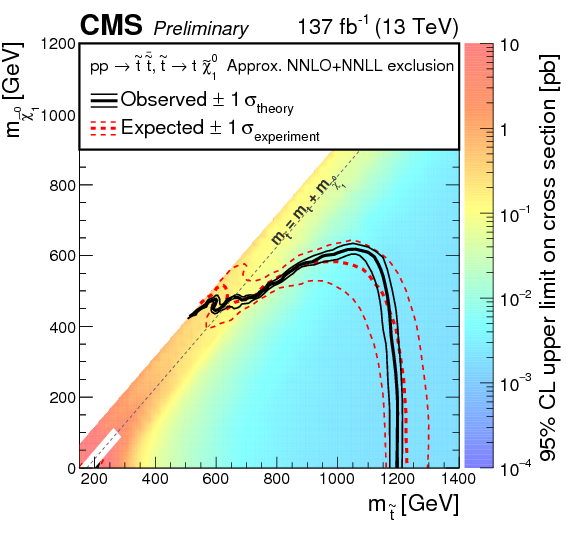
\includegraphics[width=12cm, height= 13cm]{stop_limits.png}
    \caption{The latest cross-section limit for the top squark presented in 
    \cite{cms2019search}}
    \label{fig:limits}
\end{figure}


\begin{table}
    \centering
    \begin{tabular}{c|c|c|c} 
    \toprule
    Benchmark No. & Position & $\Tilde{t}$ Mass (TeV) & $\Tilde{\chi}_1^0$ Mass (GeV) \\
    \midrule
    \rowcolor{gray!6} 1 & Outside & $ 1.2 $ & $ 600 $ \\
    2 & Outside & $ 1.225 $ & $ 400 $ \\
    \rowcolor{gray!6} 3 & Outside & $ 1.25 $ & $ 100 $ \\
    4 & Inside & $ 0.75 $ & $ 1 $\\
    \bottomrule
    \end{tabular}
    \caption{Chosen parameters for building classifiers} 
    \label{tab:benchmarks}
\end{table}